\documentclass[a4paper, 10pt]{article}

\usepackage[default]{comfortaa}
\usepackage[utf8]{inputenc}
\usepackage[english]{babel}
\usepackage{graphicx}
\usepackage{geometry}
\usepackage{titlesec}
\usepackage{multicol}
\usepackage{lastpage}
\usepackage{fancyhdr}
\usepackage{array}
\usepackage{multirow, hhline}
\usepackage[table]{xcolor}
\usepackage[hidelinks]{hyperref}
\usepackage{textcomp}

\setlength{\columnseprule}{1pt}
\setlength{\columnsep}{1cm}

\definecolor{lightgray}{gray}{0.85}

\setlength{\arrayrulewidth}{0.35mm}
\setlength{\tabcolsep}{10pt}
\renewcommand{\arraystretch}{1.7}

\fancypagestyle{plain}{%
\fancyhf{} % clear all header and footer fields
\cfoot{\thepage /\pageref{LastPage}}
\rfoot{\href{https://github.com/ElectricCanary/Bontempo}{
\includegraphics[width=5mm, height=5mm]{github}}\hspace{8pt}\href{https://www.facebook.com/ElectricCanary}{
\includegraphics[width=5mm, height=5mm]{f}}\hspace{8pt}\href{https://www.instagram.com/electricanary/}{
\includegraphics[width=5mm, height=5mm]{inst}}\hspace{12pt}\href{mailto:support@electric-canary.com}{
\includegraphics[width=5mm, height=5mm]{email}}}
\lfoot{\textcolor{black!70}{{\footnotesize\textcopyright Electric Canary - June 2020}}}
\renewcommand{\headrulewidth}{0pt}
\renewcommand{\footrulewidth}{0pt}}


\pagestyle{fancy}
\renewcommand{\headrulewidth}{0pt}
\cfoot{}
\cfoot{\thepage /\pageref{LastPage}}
\rfoot{\href{https://github.com/ElectricCanary/Bontempo}{
\includegraphics[width=5mm, height=5mm]{github}}\hspace{8pt}\href{https://www.facebook.com/ElectricCanary}{
\includegraphics[width=5mm, height=5mm]{f}}\hspace{8pt}\href{https://www.instagram.com/electricanary/}{
\includegraphics[width=5mm, height=5mm]{inst}}\hspace{12pt}\href{mailto:support@electric-canary.com}{
\includegraphics[width=5mm, height=5mm]{email}}}
\lfoot{\textcolor{black!70}{{\footnotesize\textcopyright Electric Canary - June 2020}}}
\rhead{\href{https://electric-canary.com/bontempo}{
\includegraphics[scale=0.22]{logo}}}
\lhead{\textbf{{\small\emph{\textcolor{black!70}{Bontempo-Datasheet}}}}}

\titleformat*{\section}{\huge\bfseries}
\titleformat*{\subsection}{\LARGE\bfseries}
\titleformat*{\subsubsection}{\Large\bfseries}

\geometry{hmargin=2.5cm,vmargin=2.5cm}
\headheight=35pt

\begin{document}\thispagestyle{plain}
\begin{center}
\begin{Huge}
\vspace*{0.5cm}
\textbf{Bontempo - Datasheet}
\rule {0.95\textwidth}{2pt}\\
\end{Huge}
\vspace{1cm}

\includegraphics[scale=1]{logocentre}\\
\end{center}
\vspace{1cm}
\begin{multicols}{2}
\section{Introduction}
\bigbreak
Bontempo is a precise Tap Tempo and Modulation integrated solution for PT2399 delay. It is suitable for new designs or modifying well-known PT2399 delays.\\

You can now unlock the full potential of your delay effect units. Explore new sonic territories with fully controllable modulation parameters and 6 modulation waveforms. \\

Get the exact tempo you need with the 6 Tempo divisions and calibration mode.\\

Keep your settings safe with the two user presets and the save tempo option. 
\vfill\null
\columnbreak

\section{Features}
\bigbreak
\begin{itemize}
\item \hyperref[sec:calib]{Calibrated }\hyperref[sec:digpot]{8-bit Digital Potentiometer Tap Tempo}
\item \hyperref[subsec:delaytime]{~40ms to ~1300ms Delay Time}
\item \hyperref[subsec:tempodiv]{6 Selectable Tempo Divisions} \\ 
\includegraphics[scale=1]{fourth} , 
\includegraphics[scale=1]{dotted-eight} , 
\includegraphics[scale=1]{eight} , 
\includegraphics[scale=1]{triplet} , 
\includegraphics[scale=1]{sixteenth} , 
\includegraphics[scale=1]{sextuplet}
\item \hyperref[subsec:moddepthspeed]{±30ms Max. Modulation Depth}
\item \hyperref[subsec:moddepthspeed]{~0.1Hz to ~10Hz Modulation Speed}
\item \hyperref[subsec:waveformsel]{6 Selectable Modulation Waveforms}\\ 
\includegraphics[scale=1]{sine} , 
\includegraphics[scale=1]{square} , 
\includegraphics[scale=1]{triangle} , 
\includegraphics[scale=1]{rampup} , 
\includegraphics[scale=1]{rampdown} , 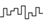
\includegraphics[scale=1]{random}
\item \hyperref[sec:userpresets]{2 User Presets}
\item \hyperref[sec:cleanmode]{Clean Mode (limits delay to 600ms for cleaner sound)}
\item \hyperref[sec:doubletime]{Double Time Mode}
\item \hyperref[sec:temposave]{Tempo EEPROM Save}
\item \hyperref[sec:dualpt]{Dual PT2399 Capability}
\item \hyperref[sec:pinconfig]{Compact DIP-14 Package}
\item \hyperref[sec:typappsche]{Minimal amount of External Parts}
\end{itemize}
\end{multicols}

\newpage
\headheight=35pt
\tableofcontents
\newpage

\section{Pin Configuration}
\label{sec:pinconfig}
\vfill
\begin{center}
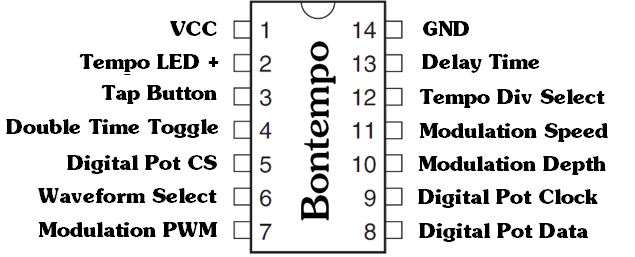
\includegraphics[scale=1]{package}
\vfill
\begin{table}[h!]
\begin{tabular}{|m{0.5cm}|m{4.5cm}|m{0.7cm}|m{7.5cm}|}
\hline
\rowcolor{lightgray} \centering {\Large\textbf{N°}} & \centering {\Large\textbf{Name}} & \centering {\Large\textbf{I/O}} & {\Large\textbf{Description}}\\
\hline
\centering 1 & \centering VCC & \centering I & Supply voltage.\\
\hline
\centering 2 & \centering Tempo LED + & \centering O & LED indicator output.\\
\hline
\centering 3 & \centering Tap Button & \centering I & Set tempo when connected  to ground.\\
\hline
\centering 4 & \centering Double Time Toggle & \centering I & Multiply tempo per 2 when connected to ground.\\
\hline
\centering 5 & \centering Digital Pot Chip Select & \centering O & Part of the SPI interface for the MCP41100 digital potentiometer.\\
\hline
\centering 6 & \centering Waveform Select & \centering I & The voltage determines the modulation waveform.\\
\hline
\centering 7 & \centering Modulation PWM & \centering O & PWM output for the MOSFET.\\
\hline
\centering 8 & \centering Digital Pot Data & \centering O & Part of the SPI interface for the MCP41100 digital potentiometer.\\
\hline
\centering 9 & \centering Digital Pot Clock & \centering O & Part of the SPI interface for the MCP41100 digital potentiometer.\\
\hline
\centering 10 & \centering Modulation Depth & \centering I & This pin's voltage determines the modulation depth between 0 and 30ms.\\
\hline
\centering 11 & \centering Modulation Speed & \centering I & This pin's voltage determines the modulation speed between 0.1 and 10Hz.\\
\hline
\centering 12 & \centering Tempo Division Select & \centering I & This pin's voltage determines the tempo division selected.\\
\hline
\centering 13 & \centering Delay Time & \centering I & This pin's voltage determines the delay time between 40 to 1300 ms if no tap sequence is active.\\
\hline
\centering 14 & \centering GND & \centering I & Ground reference voltage.\\
\hline
\end{tabular}
\caption{Pin Configuration}
\end{table}
\end{center}
\newpage

\section{Typical Application Schematic}
\label{sec:typappsche}
\bigbreak
This schematic shows how to implement the Bontempo in a simple delay project. Every options are used.
\vfill
\begin{figure} [h!]
\begin{center}
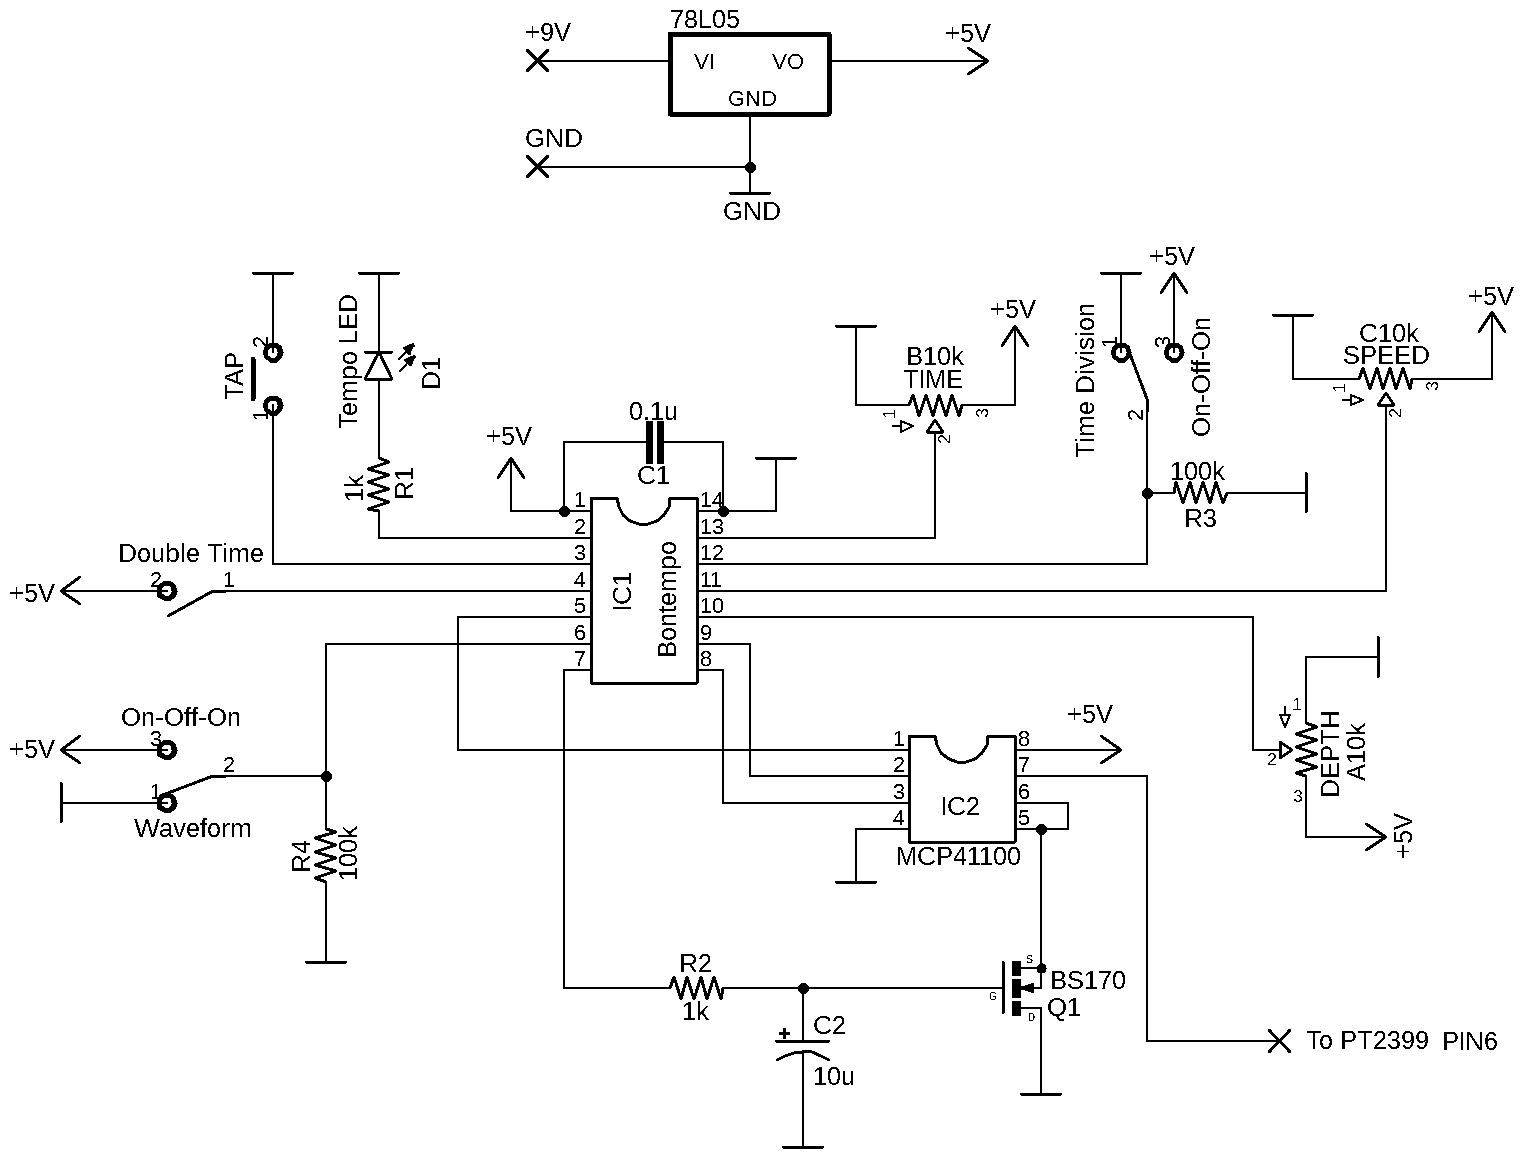
\includegraphics[scale=1.13]{Schematic}
\label{Schem}
\caption{Typical Application Schematic for a single PT2399}
\end{center}
\end{figure}
\vfill
\newpage
\section{Absolute Maximum Ratings}
\bigbreak
\begin{table}[h!]
\centering
\begin{tabular}{|c|c|}
\hline
Storage Temperature	& -65°C to +150°C\\
\hline
Operating Temperature & -55°C to +125°C\\
\hline
Voltage on any pin except pin 4	& -0.5V to Vcc + 0.5V\\
\hline
Voltage on Pin 4 & -0.5V to +13.0V\\
\hline
Maximum Operating Voltage & +6.0V\\
\hline
DC Current per I/O Pin & 40.0mA\\
\hline
DC Current VCC \& GND pins & 200.0mA\\
\hline
\end{tabular}
\caption{Absolute Maximum Ratings}
\end{table}
\bigbreak
\bigbreak
\section{DC Characteristics}
\bigbreak
\begin{table}[h!]
\centering
\begin{tabular}{|c|c|c|c|}
\hline
\rowcolor{lightgray}{\Large\textbf{Parameter}} & {\Large\textbf{Min}} & {\Large\textbf{Max}} & {\Large\textbf{Unit}}\\
\hline
Power Supply Voltage & 2.7 & 5.5 & V\\
\hline
Power Supply Current & 4.4 & 7 & mA\\
\hline
\end{tabular}
\caption{DC Characteristics}
\end{table}
\bigbreak
For any other DC characteristics please refer to the ATtiny84A \href{http://ww1.microchip.com/downloads/en/devicedoc/Atmel-7701_Automotive-Microcontrollers-ATtiny24-44-84_Datasheet.pdf}{\underline{datasheet}} (p.155).
\bigbreak
\bigbreak
\section{Specifications}

\begin{table}[h!]
\centering
\begin{tabular}{|c|c|c|c|}
\hline
\rowcolor{lightgray}{\Large\textbf{Parameter}} & {\Large\textbf{Min}} & {\Large\textbf{Max}} & {\Large\textbf{Unit}}\\
\hline
Delay Time & 37 & 1306 & ms\\
\hline
PWM frequency & - & 1 & kHz\\
\hline
Modulation Frequency & 0.12 & 10.17 & Hz\\
\hline
Modulation Depth & 0 & 30 & ms\\
\hline
All Potentiometer/Toggle Input & 0 & 5 & V\\
\hline
\end{tabular}
\caption{Specifications}
\end{table}

All specifications tested at VCC = 5V.

\section{Power Supply}
\bigbreak
The chip will operate with a power supply between 2.7V and 5.5V.
However a regulated 5.0V power supply is recommended. This is because the modulated tap tempo was calibrated at 5.0V and a change in Vcc will affect the PWM output voltage.
A 0.1$\mu$F capacitor should be connected between Vcc and GND and be placed as close to the pins as possible.\\

If using the same 5V regulator as the PT2399 be careful that the regulator can handle the extra load, and that the Bontempo is fed a correct voltage. \\

\section{Calibration}
\label{sec:calib}
\bigbreak
Unfortunately, not all digital potentiometers and BS170 are created equal. This is why a manual calibration phase is often necessary. Once completed it will be saved in EEPROM, but you can still re-calibrate if you're not satisfied.\\

For the very fist time it is the powered-up, the Bontempo will boot in Calibration Mode. Once the calibration finished, it will boot normally from now on.\\

The Tempo LED is blinking, to calibrate you need to make sure the delay is synced with the LED. You can finely adjust the delay time with the Time Pot. The Time Pot can add or subtract up to 200ms to the delay time. Once the delay is synced as close as possible to the LED Tempo you can press the Tap Button once.

Now the LED will blink slower and you can repeat the same operation. You'll need to do that 9 times before the calibration is over.\\

It is possible that, near the end of the calibration sequence, the delay time adjustment is not sufficient. This means you are hitting the maximum delay of the digital potentiometer. In that case just adjust the delay as close as possible.\\

The last step of calibration is a bit different. It is testing the maximum delay time. The Digital Pot is set at maximum delay and you can set the tempo of the LED with the Time Pot. The goal is still the same though, to synchronize the LED with the delay time.\\

If you want to be as precise as possible you can use an Oscilloscope or record the delay on a DAW. Each step increases the tempo by 100ms from 400 to 1200ms, the delay of the last step depends on the chip and circuit. 

To to re-calibrate the Bontempo, follow these instructions :\\
\begin{itemize}
\item Make sure the chip is powered down.
\item Press the Tap Button.
\item Power Up the Bontempo while keeping the Tap Button Pressed.
\item Keep the button pressed while the Tempo LED blinks once.
\item After the LED blinks twice you have 2s to release the Tap Button.
\item The LED will blink twice quickly and you are now in Calibration Mode.\\
\end{itemize}

\newpage
\section{Controls}
\subsection{Tap Tempo Button}
\bigbreak
This input is only compatible with a momentary switch.
The debounce is handled by software so no extra external components have to be used. Debounce time is 500$\mu$s.\\

The program starts counting milliseconds after the first press. The delay time tapped is in effect right after the second press of the tap button. After the second press of the tap button, every following tap in the sequence is averaged in order to reach easily the desired tempo. 

If the button is not pressed again after a certain time ,the timer is reset and the tap sequence is ended. When a tap sequence has started, it will take 2 cycles to be finished (the LED will start blinking). If the tap tempo button is pressed only once, the tap sequence will be aborted after the reset time passed (see table below).\\

\begin{table}[h!]
\centering
\begin{tabular}{|c|c|c|}
\hline
\rowcolor{lightgray}{\Large\textbf{Time Division Selected}} & {\Large\textbf{Normal}} & {\Large\textbf{Clean Mode}}\\
\hline

\includegraphics[scale=1.2]{fourth} & 2.1s & 1.4s\\
\hline

\includegraphics[scale=1.2]{dotted-eight} & 2.5s & 1.6s\\
\hline

\includegraphics[scale=1.2]{eight} & 3.4s & 2s\\
\hline

\includegraphics[scale=1.2]{triplet} & 4.7s & 2.6s\\
\hline

\includegraphics[scale=1.2]{sixteenth} & 6s & 3.2s\\
\hline

\includegraphics[scale=1.2]{sextuplet} & 8.6s & 4.4s\\
\hline
\end{tabular}
\caption{Tap Sequence Reset Time}
\end{table}

The reset time follows this equation: $\frac{Max Delay}{Tempo Div Mult} + 800 = Reset Time (ms)$\\

Max Delay is around 1300ms in normal mode and 600ms in clean mode. Tempo Div Mult is the multiplier of the current time division (1, 0.75, 0.5, 0.33, 0.25, 0.17).\\

When the tap tempo is active, the tempo LED will blink with the rhythm you tapped, regardless of the selected tempo division.\\

\subsection{Delay Time}
\label{subsec:delaytime}
\bigbreak
This input is to voltage control the delay time. This input will control the delay time until you activate the tap tempo. While the delay time is controlled by this input, the Tempo LED and Scale LED will stay on.\\

To take back control from the Tap Tempo, you just need to modify this input's voltage by 5\%.Typically, you would use a Potentiometer for the delay time control. The recommended potentiometer value is 10k$\Omega$ or above, to avoid having too much current going through the pin.\\

You can add a 0.1$\mu$F capacitor between the input and ground for smoother time changes.\\

\subsection{Tempo Division Select}
\label{subsec:tempodiv}
\bigbreak
Six different tempo division are accessible with this input. To access every time division a SPDT On-Off-On toggle switch is required.\\

The first three time divisions are fourth, dotted eighth and eighth. The last three time divisions are accessed by first pressing the tap button and then changing the toggle position while the tap button is pressed. The press will not count as a press for the tap tempo. The three last time divisions are triplet, sixteenth and sextuplet.\\

The time divisions are selected by changing the Tempo Div Select Pin's voltage (Pin 12).\\

\begin{table}[h!]
\centering
\begin{tabular}{|c|l|l|}
\hline
\rowcolor{lightgray} & \multicolumn{2}{c|}{{\Large\textbf{Tempo Division}}}\\
\hhline{|>{\arrayrulecolor{lightgray}}->{\arrayrulecolor{black}}|--|}
\rowcolor{lightgray}\multirow{-2}{5cm}{\centering{\Large\textbf{Pin 12 Voltage}}} & {\centering\large\textbf{Not Pressed}} & {\centering\large\textbf{Button Pressed}}\\
\hline
GND - 0.39V & Fourth \hfill \includegraphics[scale=1]{Fourth} & Triplet \hfill 
\includegraphics[scale=1]{triplet}\\
\hline
0.4V - 4.4V & Dotted-Eighth \hfill 
\includegraphics[scale=1]{dotted-eight}& Sixteeth \hfill 
\includegraphics[scale=1]{sixteenth}\\
\hline
4.5V - 5V & Eighth \hfill 
\includegraphics[scale=1]{eight} & Sextuplet \hfill 
\includegraphics[scale=1]{sextuplet}\\
\hline
\end{tabular}
\caption{Modulation Waveform Selection}
\end{table}

If the time division is changed while the Tap Tempo is active, the delay time will be changed accordingly instantly.\\

You can access the middle time division by putting a resistor between pin 12 and ground. Any value between 5k$\Omega$ and 140k$\Omega$ would potentially work, but a 100k$\Omega$ resistor is recommended in order not to draw too much current.\\


\subsection{Modulation Depth \& Speed}
\label{subsec:moddepthspeed}
\bigbreak
Same recommendations than the Delay Time (10k$\Omega$ or more, 0.1$\mu$F capacitor …).\\

Modulation speed goes from 0.12Hz to 10.17Hz. Modulation depth maximum is 30ms.\\

\subsection{Modulation Waveform Select}
\label{subsec:waveformsel}
\bigbreak
Six different modulation waveforms are accessible with this input. To access every waveform a SPDT On-Off-On toggle switch is required. 
The first three waveforms are sine, square and triangle. The last three waveforms are accessed by first pressing the tap button and then changing the toggle position while the tap button is pressed. The press will not count as a press for the tap tempo. The last three modulation waveforms are Ramp-up, Ramp-Down and Random.\\

The modulation waveforms are selected by changing the Modulation Waveform Select Pin's voltage (Pin6).\\
\newpage
\begin{table}[h!]
\centering
\begin{tabular}{|c|l|l|}
\hline
\rowcolor{lightgray} & \multicolumn{2}{c|}{{\Large\textbf{Waveform}}}\\
\hhline{|>{\arrayrulecolor{lightgray}}->{\arrayrulecolor{black}}|--|}
\rowcolor{lightgray}\multirow{-2}{5cm}{\centering{\Large\textbf{Pin 6 Voltage}}} & {\centering\large\textbf{Not Pressed}} & {\centering\large\textbf{Button Pressed}}\\
\hline
GND - 0.39V & Sine \hfill 
\includegraphics[scale=1]{sine} & Ramp-Up \hfill 
\includegraphics[scale=1]{rampup}\\
\hline
0.4V - 4.4V & Square \hfill 
\includegraphics[scale=1]{square}& Ramp-Down \hfill 
\includegraphics[scale=1]{rampdown}\\
\hline
4.5V - 5V & Triangle \hfill 
\includegraphics[scale=1]{triangle} & Random \hfill 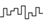
\includegraphics[scale=1]{random}\\
\hline
\end{tabular}
\caption{Modulation Waveform Selection}
\end{table}
The waveforms can sound a bit asymmetrical at high modulation depth, this is due to the MOSFET’s non-linearity. \\

Like for the Time Division Toggle, a 100k$\Omega$ resistor is recommended to access the middle waveform.\\

\subsection{Double Time}
\label{sec:doubletime}
\bigbreak
The double time divide the time division multiplier per two. This results in tempo that's two time faster. This effect is not affected by preset recall. Double Time has no effect on the Delay Time when controlled by the Delay Time input.
This effect can be used dynamically or just set as wanted.\\

When the Double Time Pin (Pin 4) is connected to Vcc, the double time mode is active. If the Double Time Pin is connected to Ground, the double time mode is disabled.\\ 
\newpage
\section{User Presets}
\label{sec:userpresets}
\bigbreak
You can easily save and recall two user presets on the Bontempo. These presets are saved on the Bontempo's EEPROM so that they can survive the power cycles.\\

To recall preset 1 you must:\\
\begin{itemize}
\item Push the Tap Button and keep it pressed for 3s.
\item After the LED blinks once, release the Tap Button.
\item The LED will blink once quickly and preset 1 is recalled.\\
\end{itemize}

To recall preset 2 you must:\\
\begin{itemize}
\item Push the Tap Button and keep it pressed for 3s.
\item Keep it pressed while the LED blinks once.
\item After the LED blinks twice, release the Tap Button.
\item The LED will blink twice again quickly and preset 2 is recalled.\\
\end{itemize}

To save preset 1 you must:\\
\begin{itemize}
\item Push the Tap Button and keep it pressed for 3s.
\item Keep it pressed while the LED blinks once.
\item Keep it pressed while the LED blinks twice.
\item After the LED "reverse-blinks" once, release the  Tap Button.
\item The LED will "reverse-blink" once again quickly and preset 1 is now saved.\\
\end{itemize}

To save preset 2 you must:\\
\begin{itemize}
\item Push the Tap Button and keep it pressed for 3s.
\item Keep it pressed while the LED blinks once.
\item Keep it pressed while the LED blinks twice.
\item Keep it pressed while the LED "reverse-blinks" once.
\item After the LED "reverse-blinks" twice, release the  Tap Button.
\item The LED will "reverse-blink" twice again quickly and preset 2 is now saved.\\
\end{itemize}

Keep in mind that, unfortunately, the Feedback setting in delay circuits cannot be saved since it's not controlled by the Bontempo.

Furthermore, the double time toggle cannot be saved in presets but will still affect the tempo even when a preset is recalled. This applies for the clean mode too.\\

The tempo (tapped or set with a potentiometer), the tempo division, the modulation speed, modulation depth and modulation waveform can be saved and recalled at will.

The recalled tempo will not take the clean mode into account.\\

Once you recall a preset, any parameters can be changed without affecting the other preset's parameters.\\

\section{Tempo Save}
\label{sec:temposave}
\bigbreak
When you tap a tempo it is saved on the Bontempo's EEPROM. This means that if you power down the Bontempo while a tap sequence is active, the Bontempo will resume this sequence when powered up. This is true even if some parameters are moved when the Bontempo is powered down.\\
\section{Clean Mode}
\label{sec:cleanmode}
\bigbreak
The clean mode limits the maximum tempo to 600ms. This will produce a less distorted delay. This will emulate a 50k$\Omega$ time potentiometer, like some PT2399 delay.
\bigbreak
To activate the Clean Mode, you need to:
\begin{itemize}
\item Make sure the chip is powered down.
\item Press the Tap Button.
\item Power Up the Bontempo while keeping the Tap Button Pressed.
\item Keep the button pressed until the Tempo LED blinks once.
\item You now have 2s to release the button, the LED will blink   once again quickly.
\item You are now in Clean Mode.
\end{itemize}
\bigbreak
This status is written in the chip's EEPROM. This mean the Bontempo will boot in clean mode every time.
To deactivate Clean Mode, just repeat the procedure above. The chip will now boot in normal mode every time.\\

\section{Deactivating Modulation}
\bigbreak
If you don’t wish to use the modulation features, just connect Waveform Select Pin (Pin 6), Modulation Depth (Pin 10) and Modulation Speed (Pin 11) to ground.\\

Do not disconnect the BS170 MOSFET !\\

The BS170 is taken into account during the calibration. Discarding the MOSFET will result in extremely imprecise tap sequences.\\
\newpage
\section{Digital Potentiometer SPI Interface}
\label{sec:digpot}
\bigbreak
The only digital potentiometer guaranteed to work are the MCP41100 and MCP42100. They are 8bit 100kΩ SPI controlled digital potentiometers. The SPI interface requires 3 pins (Clock, Data and Chip Select). Since the potentiometer is 8bit, it has 256 different wiper positions. This limits the tempo precision to approximately 5ms. For more information about the digital potentiometers see the \href{http://ww1.microchip.com/downloads/en/DeviceDoc/11195c.pdf}{\underline{datasheet}}.\\

Please be careful with the connection between the digital potentiometer and the PT2399, as the PT2399 is sensible to noise and this could throw off the calibration. Keep the connection short and direct.\\

\section{PWM Output}
\bigbreak
Modulation and precision compensation on the Bontempo is achieved by outputting a voltage to a BS170 MOSFET in series with the digital potentiometer. The PWM frequency is 1kHz, since this frequency is the audible spectrum, we need to filter it. If a filter is not used it will result in some ring modulation in the modulated delay signal.\\

The chip is calibrated with a first order filter composed of a 1k$\Omega$ resistor and a 10$\mu$F capacitor. The 1kHz is reduced by 36dB by this filter, which is sufficient to the ring modulation inaudible.\\

\section{Dual PT2399 Operation}
\label{sec:dualpt}
\bigbreak
If you wish to use the Bontempo in a dual PT2399 design, the Double Time Toggle Pin will become a "Half-Time Toggle Pin". If you don't wish to use this feature dynamically, just connect Pin4 to Vcc. \\

%\begin{figure}[h!]
%\centering
%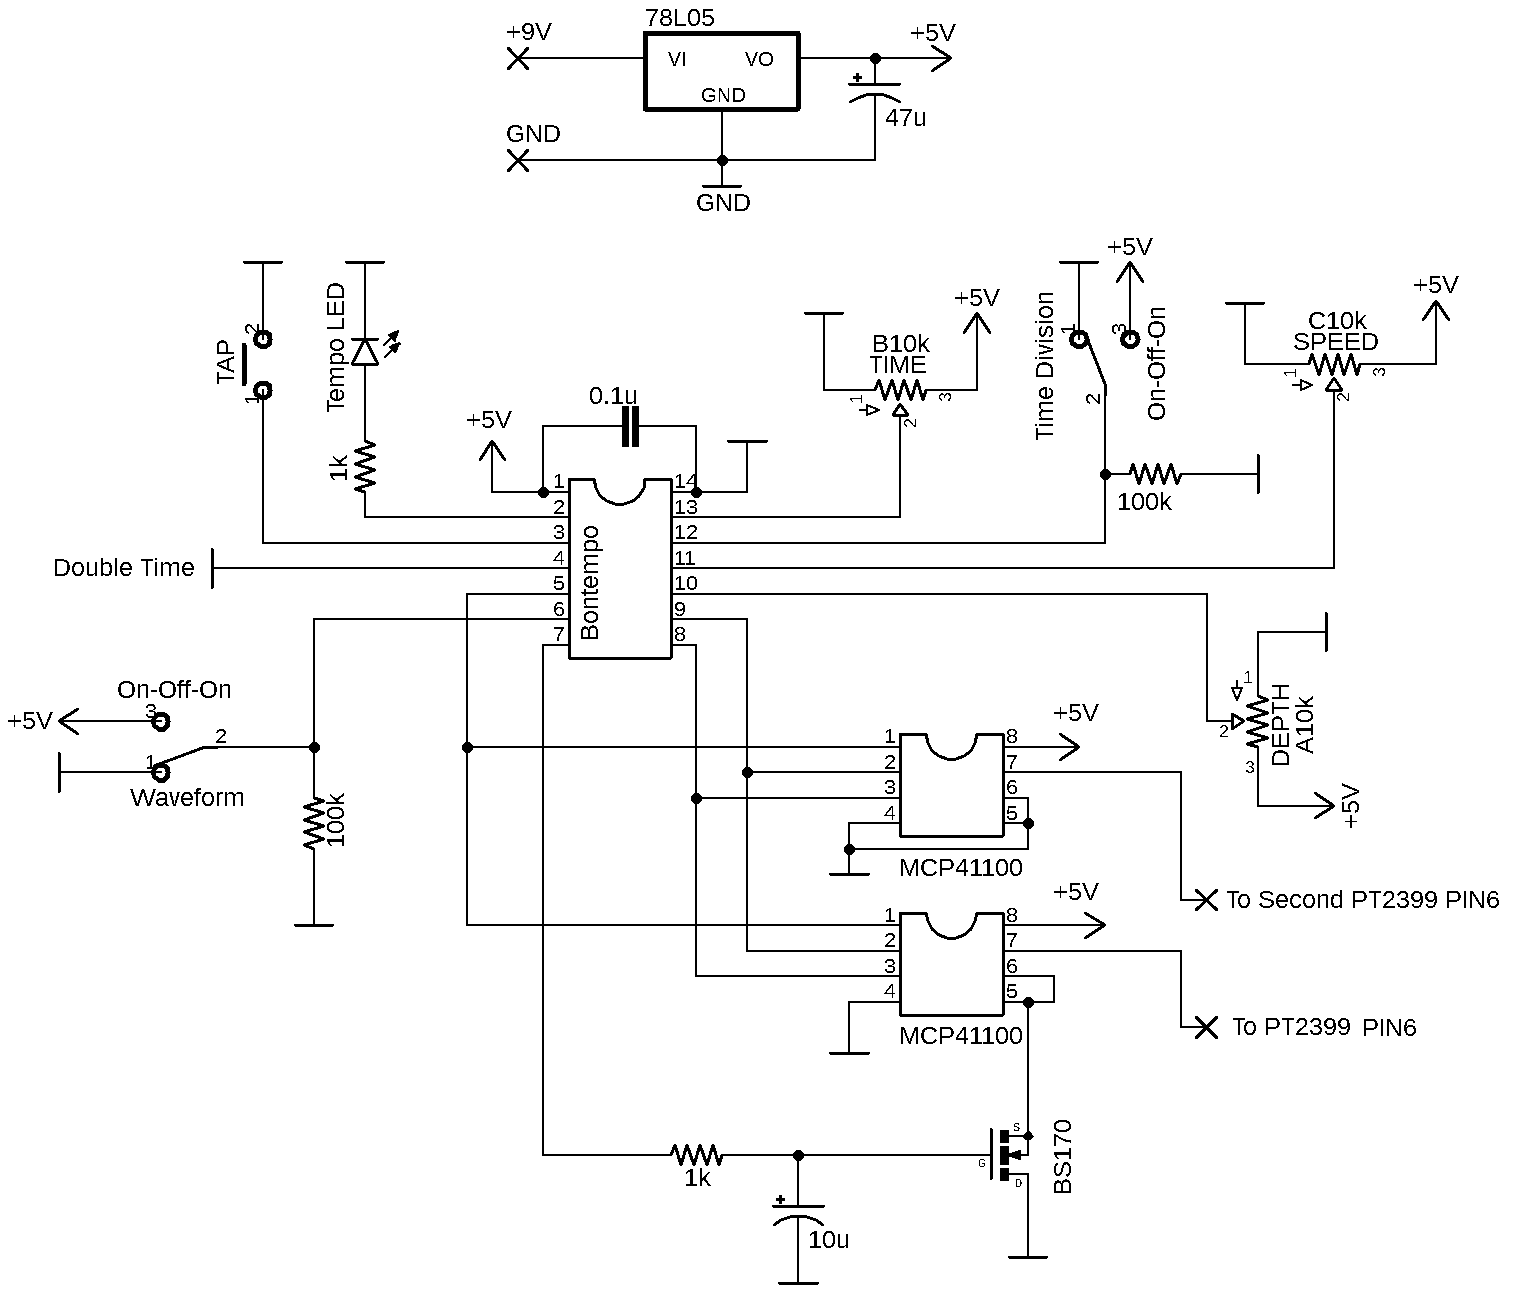
\includegraphics[scale=0.7]{DualSchematic}
%\caption{Typical Application Schematic for Dual PT2399 Operation}
%\end{figure}

\section{Tempo LED}
\bigbreak
When the delay time is controlled by the Delay Time input the LED will stay on.\\

When tapping a tap sequence, the LED will blink exactly when you press the tap button, beginning with the second press.\\

When the Tap Tempo is active, the tempo LED will blink in sync with the tempo you tapped regardless of the tempo division selected. During the blinking phase, the LED stays on for 8ms.\\

\end{document}
